\subsection{Client}
Diese Komponente enthält die eigentliche Repräsentation einer Partie, die sowohl von einem Spieler, als auch von einem Beobachter, jedoch in reduzierter Form genutzt werden soll.

\subsubsection{Schnittstellenarten}
Als Benutzerschnittstelle ist eine grafische Benutzeroberfläche zu verwenden. \\ \textbf{Begründung:} Bei der Spielansicht handelt es sich um die zentrale Komponente der Client-Anwendung. Über diese interagiert ein Nutzer mit dem Spiel. Um das Spiele so intuitiv wie möglich zu gestalten ist es sinnvoll alle für das Spielgeschehen relevanten Informationen und Aktionen Grafisch aufzubereiten und in einer GUI dem Nutzer Bereit zu stellen. 

\subsubsection{Dialoge}
Im Folgenden sind alle Dialoge, welche während der Nutzung erscheinen können, den zugehörigen Anwendungsfällen zugeordnet. Dabei wird auf die Dialog \textit{Pause} und \textit{Spielende} im Abschnitt zum \textit{Client Hauptmenü} genauer eingegangen.

\begin{figure}[H]
    \centering
    \begin{tabular}{| l l l l |}
    	\hline
    	\textbf{Name} & \textbf{Typ} & \multicolumn{2}{l|}{\textbf{Abgedeckte Anwendungsfälle}} \\\hline
    	Spiel & Dialog & & sieh Hauptmenü -> Spiel Dialog\\\hline
    	Pause & Dialog & & sieh Hauptmenü -> Pause Dialog\\\hline
    	Spielende & Dialog & & sieh Hauptmenü -> Spielende Dialog\\\hline
    	Ungültiger Zug & Benachrichtigung & FA67 & Eingabeverarbeitung \\\hline
    	Partie Überlänge & Benachrichtigung & FA52 & Überlängenbehandlung \\\hline
    	Tor & Benachrichtigung & FA8 & Punkte erzielen \\\hline
    	Schnatz gefangen & Benachrichtigung & FA30 & Schnatz fangen \\\hline
    	Faul & Benachrichtigung & FA37 & Fouls \\\hline
    \end{tabular}
\end{figure}

\subsubsection{Dialogstrukturdiagramme} 
	%@TODO Bla Bla    
	\begin{figure}[H]
    	\centering
    	%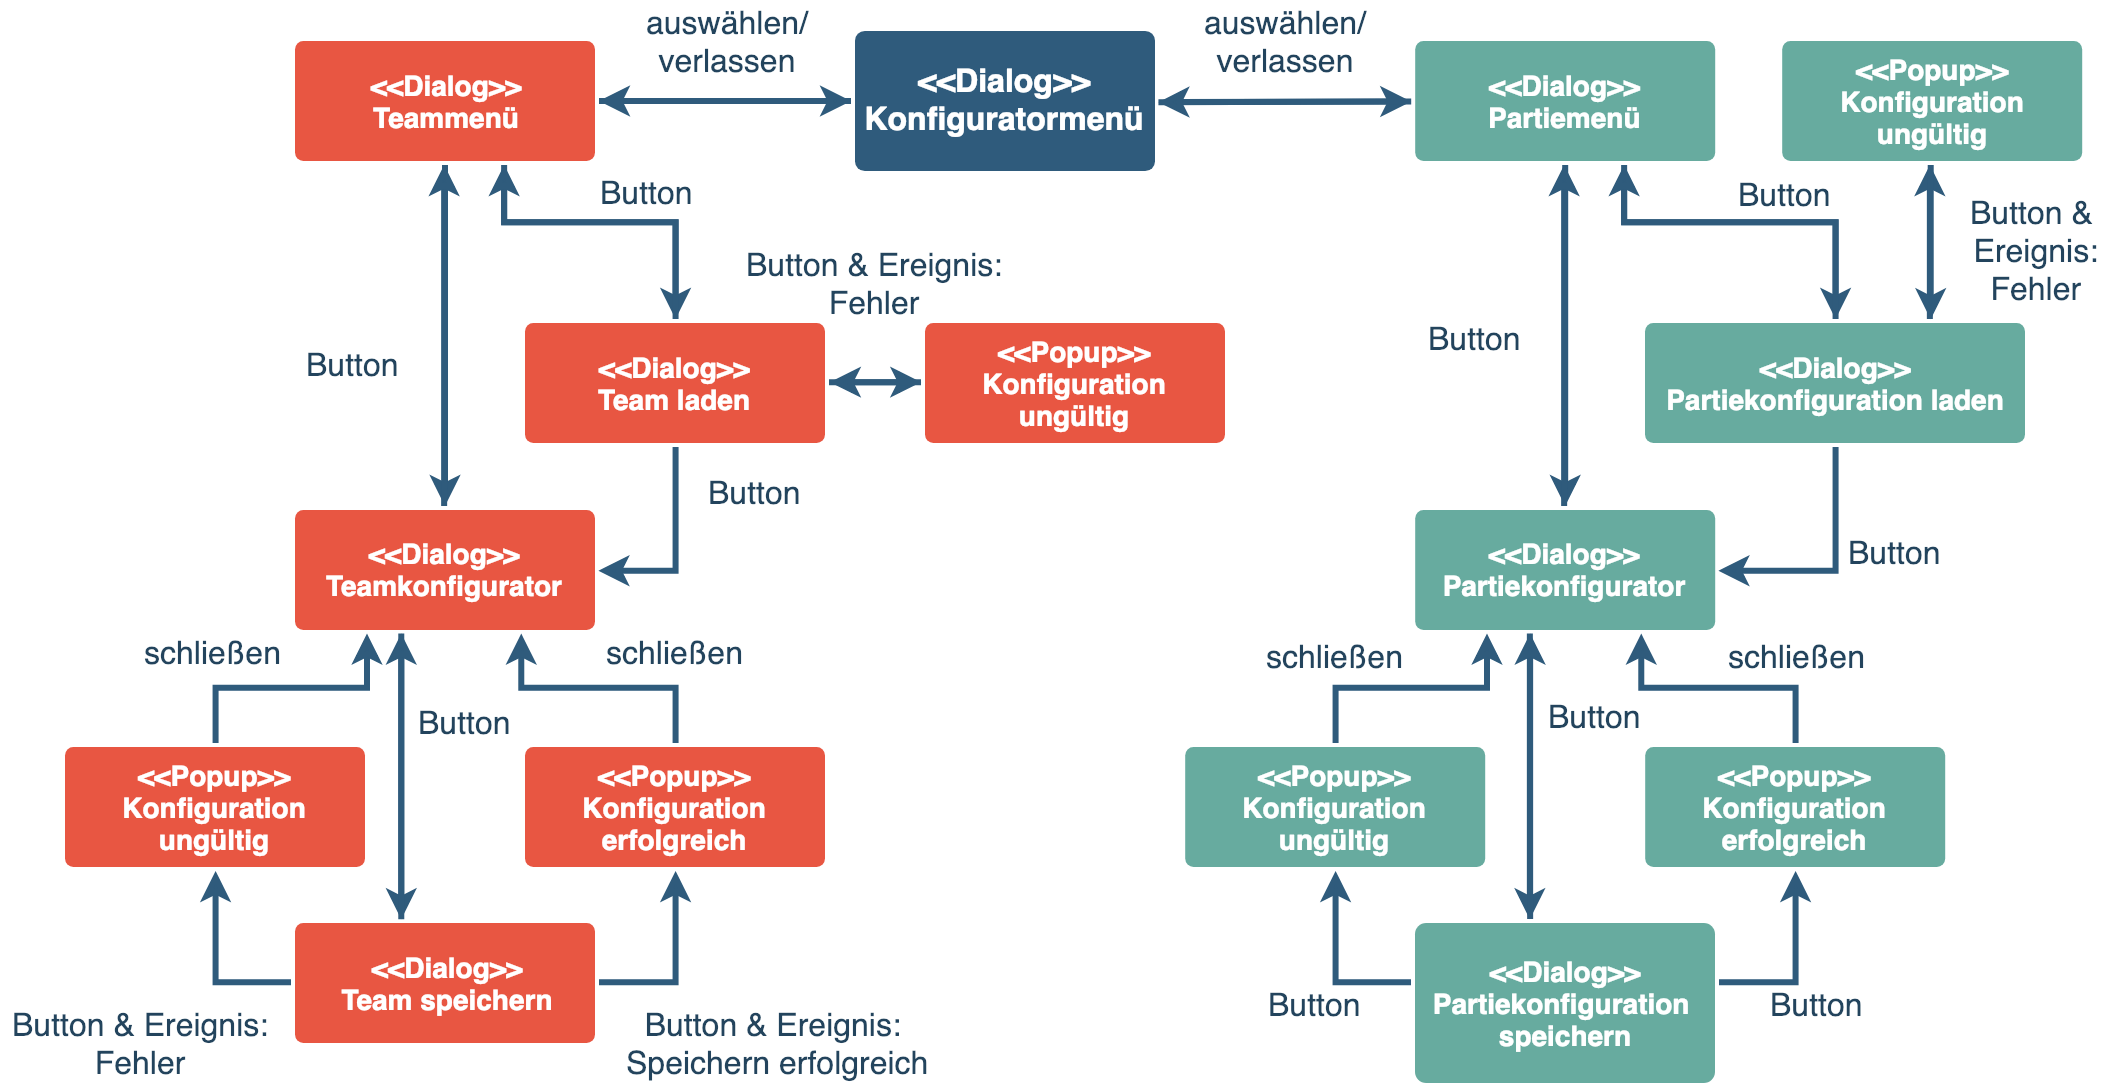
\includegraphics[width=\textwidth]{images/dialogstruktur_konfigurator}
	\end{figure}



